\begin{figure}[H]
  \begin{subfigure}[t]{0.48\linewidth}
    \centering
    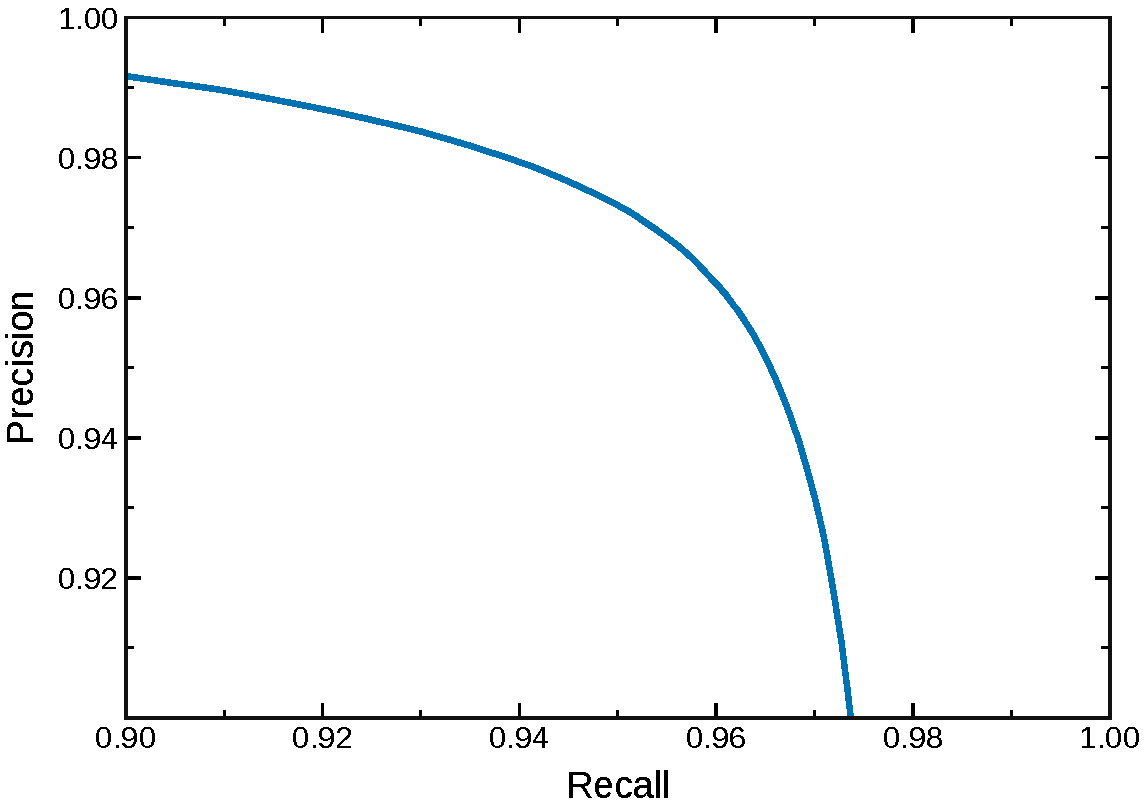
\includegraphics[width=\linewidth]{figures/methods/01_particle_detection_pr_curve_seed260745.pdf}
    \caption{}
  \end{subfigure}
  \hfill
  \begin{subfigure}[t]{0.48\linewidth}
    \centering
    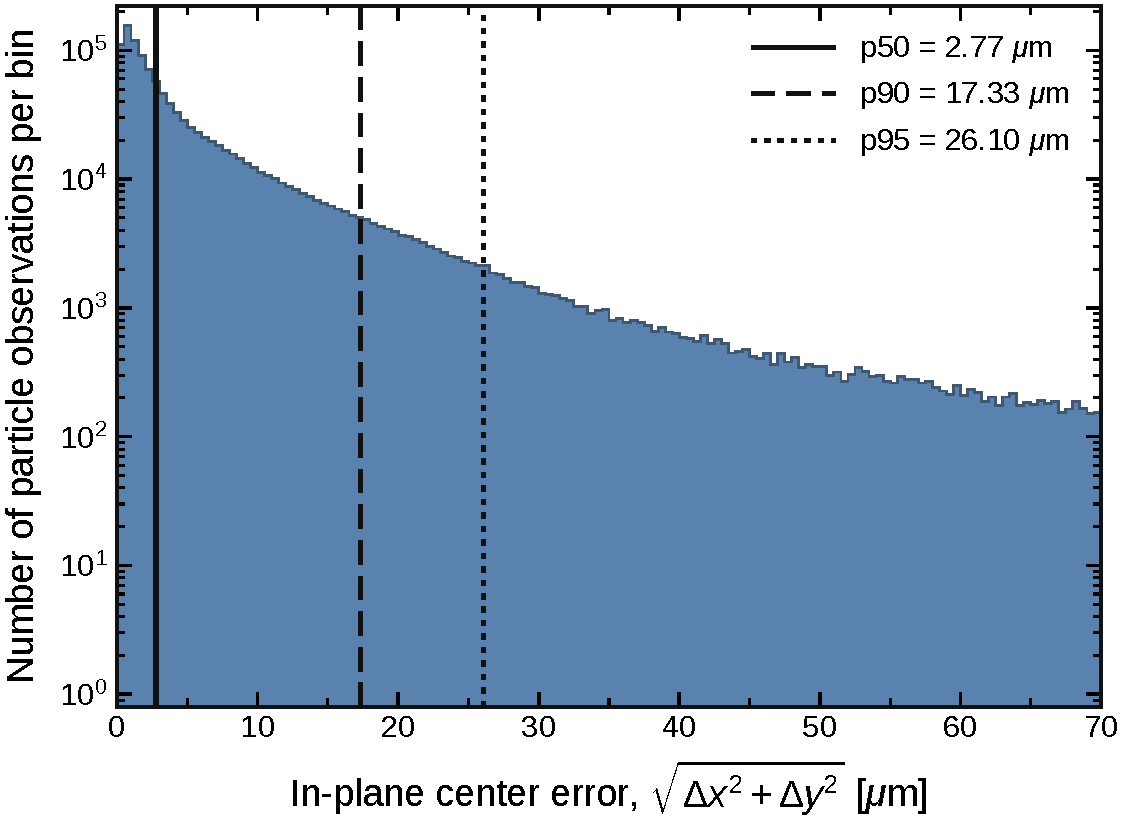
\includegraphics[width=\linewidth]{figures/methods/02_xy_center_error_smoothed_hist_seed260745.pdf}
    \caption{}
  \end{subfigure}

  \medskip

  \begin{subfigure}[t]{0.48\linewidth}
    \centering
    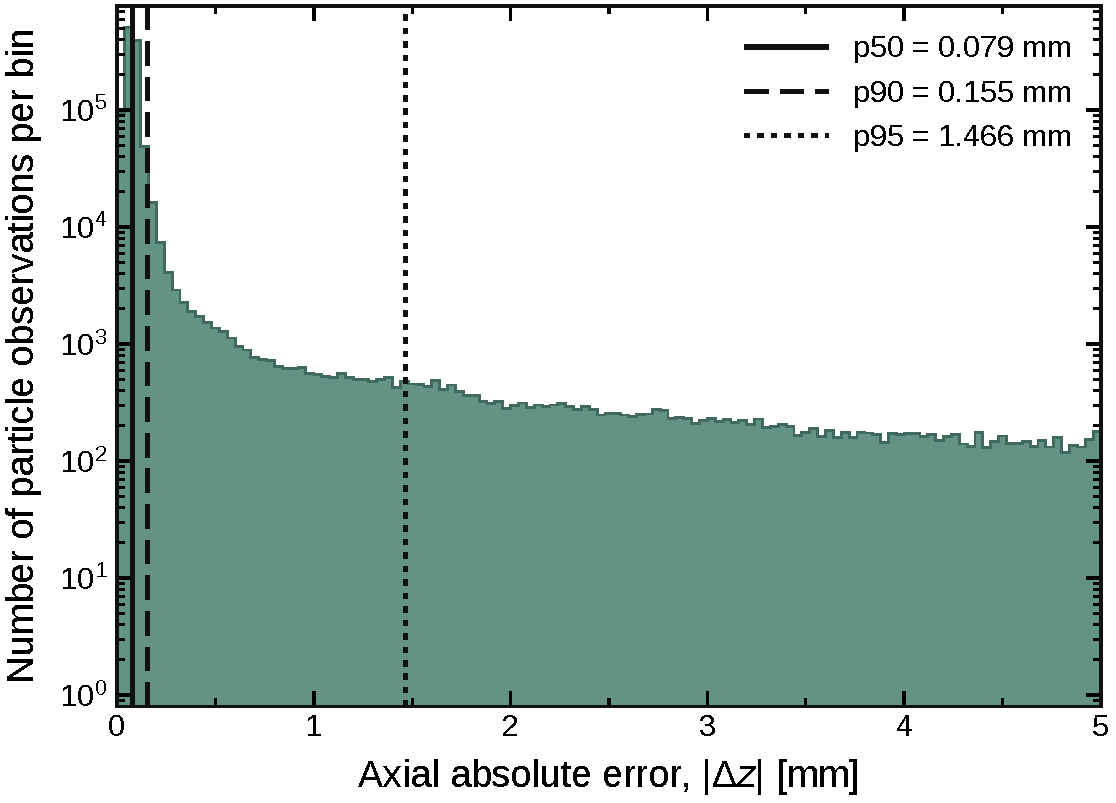
\includegraphics[width=\linewidth]{figures/methods/03_axial_error_smoothed_hist_seed260745.pdf}
    \caption{}
  \end{subfigure}
  \hfill
  \begin{subfigure}[t]{0.48\linewidth}
    \centering
    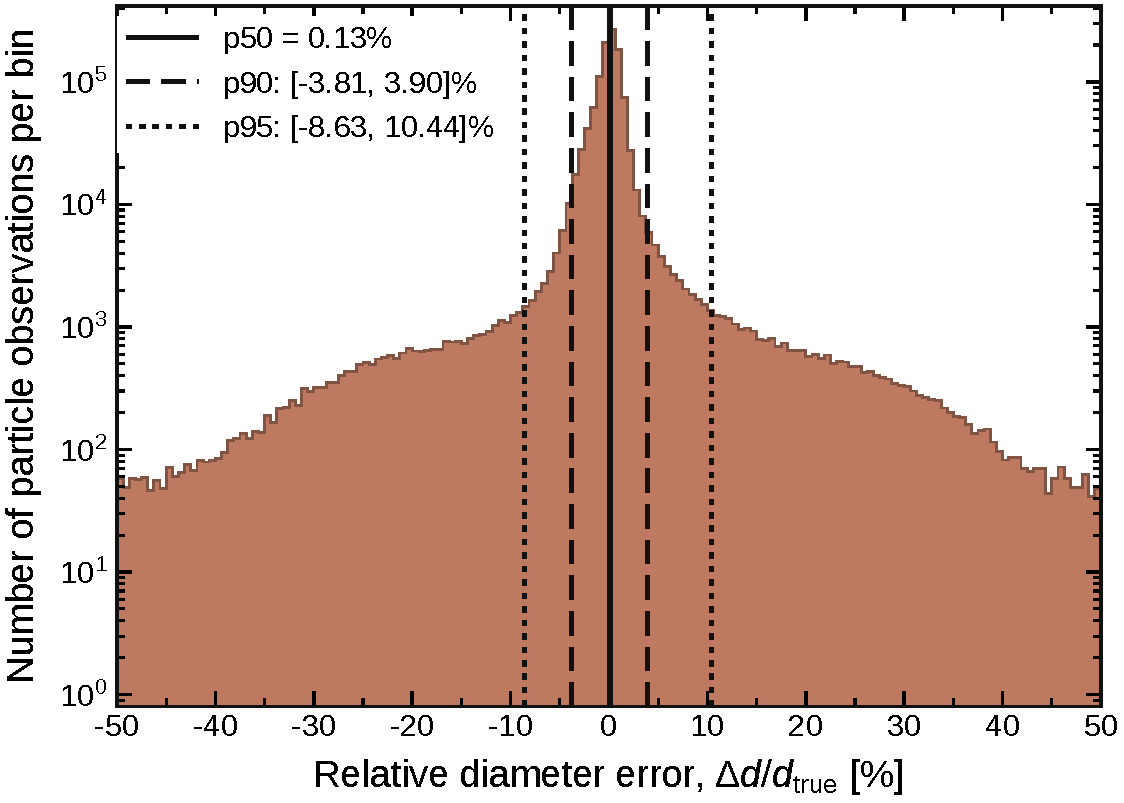
\includegraphics[width=\linewidth]{figures/methods/04_diameter_relative_error_hist_seed260745.pdf}
    \caption{}
  \end{subfigure}

  \medskip

  \begin{subfigure}[t]{0.48\linewidth}
    \centering
    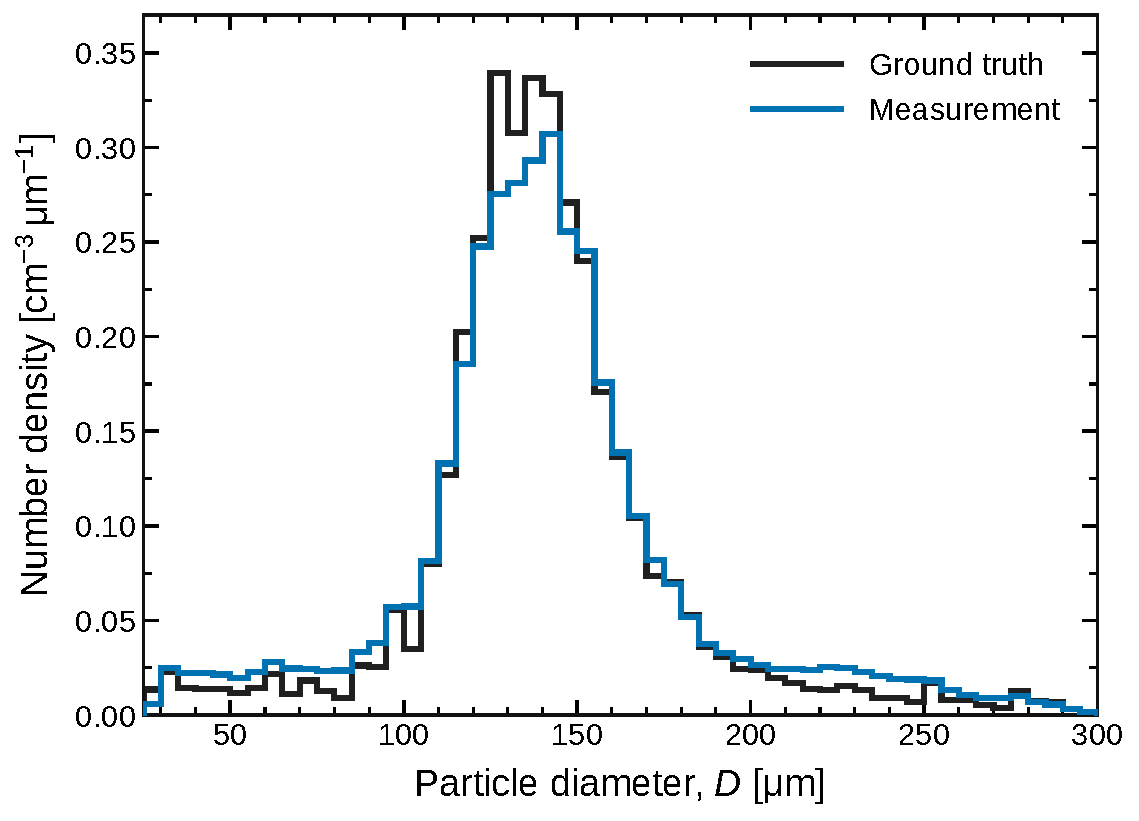
\includegraphics[width=\linewidth]{figures/methods/paper_number_density_distribution_25_300um_seed260745.pdf}
    \caption{}
  \end{subfigure}
  \hfill
  \begin{subfigure}[t]{0.48\linewidth}
    \centering
    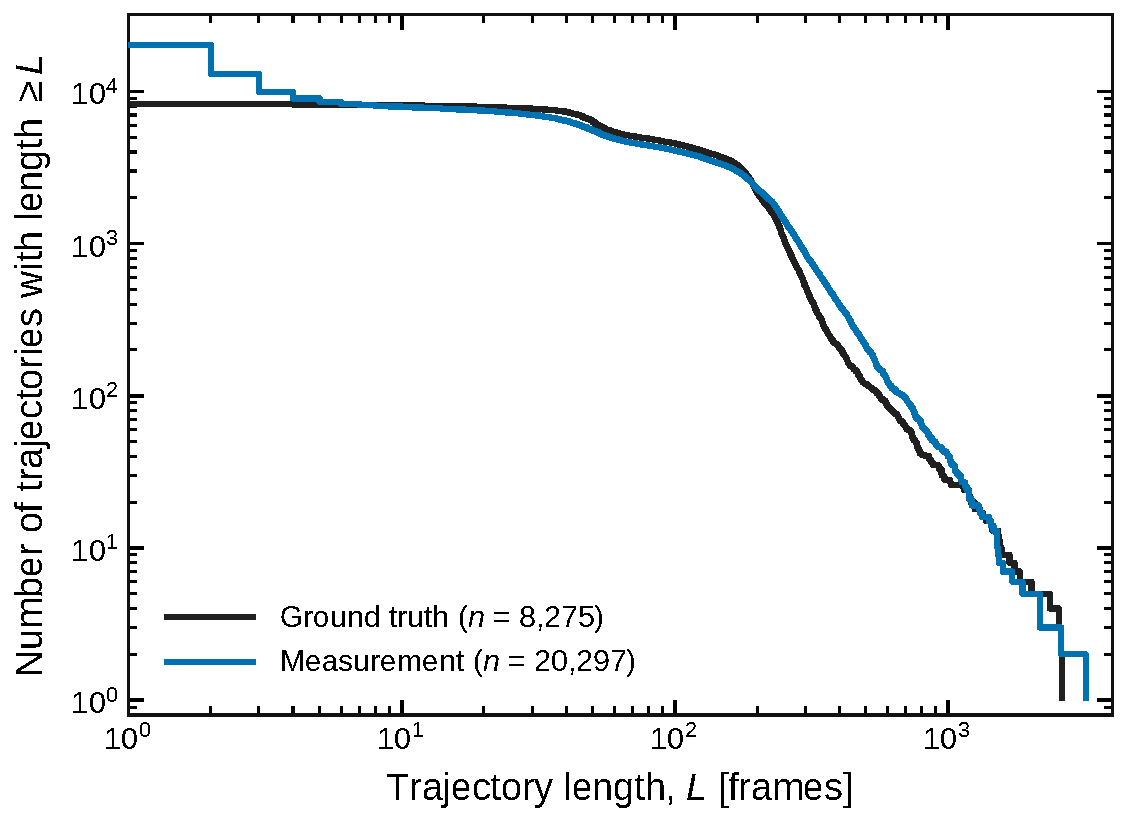
\includegraphics[width=\linewidth]{figures/methods/paper_trajectory_length_counts_25_300um_seed260745.pdf}
    \caption{}
  \end{subfigure}
  \caption{Performance of holographic droplet detection and tracking using HoloD3\cite{HoloD3} on the synthetic test sequence. (a) Particle-level precision--recall curve. Histograms show (b) the in-plane position error, \(\sqrt{\Delta x^2+\Delta y^2}\), (c) the absolute axial-position error, \(|\Delta z|\), and (d) the signed relative diameter error, \(100(D_{\mathrm{meas}}-D_{\mathrm{true}})/D_{\mathrm{true}}\). Annotations in (b,c) report the 50th, 90th, and 95th percentiles; those in (d) report the median and central 90\% and 95\% intervals. (e) Ground-truth and measured number-density distributions. (f) Cumulative numbers of trajectories with length greater than or equal to \(L\), for the ground-truth and reconstructed trajectories.}
  \label{fig:synthetic_hologram_distribution}
\end{figure}
